\documentclass[conference]{IEEEtran}

\usepackage{cite}
\usepackage{amsmath,amssymb}
\usepackage{graphicx}
\usepackage{booktabs}
\usepackage{multirow}
\usepackage{url}
\usepackage{float}
\usepackage{xcolor}

\newcommand{\rankfirst}[1]{\textcolor{blue}{#1}}
\newcommand{\ranksecond}[1]{\textcolor{red}{#1}}

\begin{document}

\title{Efficient LayerNorm-Gated Spectral-Spatial Attention Network for Multi-Scale Single Image Super-Resolution}

\author{
\IEEEauthorblockN{Stevano Titondea Prayoga Putra}
\IEEEauthorblockA{Department of Informatics Engineering\\
Dian Nuswantoro University\\
Semarang, Indonesia\\
stevanoputra38@gmail.com}
\and
\IEEEauthorblockN{Guruh Fajar Shidik}
\IEEEauthorblockA{Department of Informatics Engineering\\
Dian Nuswantoro University\\
Semarang, Indonesia\\
guruh.fajar@research.dinus.ac.id}
}

\maketitle

\begin{abstract}
Single image super-resolution (SISR) aims to reconstruct a high-resolution image from a low-resolution observation. Although recent deep networks have improved reconstruction accuracy, many designs increase model complexity and inference cost, which limits their practical use across multiple upscaling factors. This paper presents GSA-LN, an efficient spectral-spatial attention network for multi-scale SISR. Instead of positioning the model as a general state-of-the-art replacement, this study focuses on the balance between reconstruction quality, parameter efficiency, and stable multi-scale behavior. GSA-LN combines an EDSR-style residual backbone without batch normalization, frequency-aware channel attention, decomposed large-kernel spatial attention, learnable frequency attention, contrast-aware pixel refinement, and learnable residual scaling. The model is trained on DF2K and evaluated on standard bicubic SISR benchmarks, including Set5, Set14, BSD100, Urban100, and Manga109, for scale factors x2, x3, and x4. Experimental results show competitive PSNR values with only 2.6M to 3.1M parameters, reaching 38.14 dB on Set5 x2, 34.56 dB on Set5 x3, and 32.34 dB on Set5 x4. These results indicate that spectral-spatial attention can provide a practical accuracy-efficiency trade-off for conventional SISR benchmarks.
\end{abstract}

\begin{IEEEkeywords}
single image super-resolution, efficient deep learning, spectral attention, large kernel attention, LayerNorm, multi-scale reconstruction
\end{IEEEkeywords}

\section{Introduction}

Single image super-resolution (SISR) is a low-level computer vision task that reconstructs a high-resolution (HR) image from a low-resolution (LR) input. The problem is ill-posed because multiple HR images may correspond to the same LR observation after degradation. Deep convolutional networks have become a dominant solution for SISR because they can learn nonlinear LR-to-HR mappings from paired training data. However, improving reconstruction quality often comes with deeper backbones, stronger attention modules, or transformer-based components that increase computational cost.

For practical SISR, especially when the same design is expected to work across x2, x3, and x4 upscaling, the objective should not be limited to maximizing PSNR. A useful model should also remain compact, trainable, and consistent across benchmark datasets. This motivates a safer research framing: rather than claiming a universal state-of-the-art architecture, this study investigates whether a compact spectral-spatial attention design can provide competitive reconstruction quality under a moderate parameter budget.

The proposed GSA-LN network follows this direction. It uses a residual convolutional backbone without batch normalization to preserve feature flexibility, then applies three complementary forms of attention. First, frequency-aware channel attention extracts channel descriptors from the FFT magnitude of intermediate features. Second, large kernel attention (LKA) approximates a wide spatial receptive field using decomposed depth-wise convolutions. Third, learnable frequency attention uses content-aware frequency descriptors to modulate spectral responses. A contrast-aware pixel attention (CAPA) module further refines high-contrast regions before reconstruction, while learnable residual scaling controls feature fusion before upsampling.

The contributions of this paper are summarized as follows:
\begin{itemize}
    \item We reformulate GSA-LN as an efficient multi-scale SISR model that emphasizes an accuracy-efficiency trade-off instead of an overgeneralized state-of-the-art claim.
    \item We integrate frequency-aware channel attention, decomposed large-kernel spatial attention, learnable frequency modulation, CAPA, and learnable residual scaling into a compact residual SISR architecture.
    \item We evaluate the model on standard bicubic SISR benchmarks across x2, x3, and x4 scales, reporting PSNR and parameter counts to support a practical comparison.
    \item We discuss the empirical boundaries of the current evaluation and outline additional efficiency and ablation measurements needed for a more complete assessment.
\end{itemize}

\section{Related Work}

\subsection{CNN-Based Super-Resolution}

Early deep SISR models showed that convolutional neural networks can directly learn LR-to-HR mappings. SRCNN introduced an end-to-end CNN formulation for image super-resolution \cite{dong2016srcnn}, while VDSR improved reconstruction by learning residual images with a deeper network \cite{kim2016vdsr}. EDSR further improved performance by removing batch normalization from residual blocks and increasing representational capacity \cite{lim2017edsr}. These CNN-based models remain important baselines because they provide strong reconstruction performance with relatively simple architectures.

\subsection{Attention and Efficient SISR}

Attention mechanisms have been widely used to improve feature selectivity in SISR. Channel attention, spatial attention, and non-local attention can help a network focus on informative image structures, but they may also increase complexity. RCAN uses residual channel attention to model channel-wise dependencies \cite{zhang2018rcan}, while later methods explore non-local or transformer-style dependencies for broader spatial context \cite{liu2020nlsn,liang2021swinir}. In parallel, lightweight SISR models such as IMDN, RFDN, MADNet, and other compact networks show the importance of balancing PSNR, parameter count, and runtime \cite{hui2019imdn,liu2020rfdn,lan2021madnet}. This paper follows the efficient SISR direction by using compact convolutional attention components rather than a heavy transformer backbone.

\subsection{Frequency-Aware Reconstruction}

SISR quality is strongly affected by high-frequency details such as edges, textures, and repeated structures. Conventional spatial convolutions may oversmooth these components, especially at higher upscaling factors. Frequency-aware processing provides a complementary view by explicitly analyzing spectral magnitudes or frequency bands. In GSA-LN, the frequency domain is used in two ways: as a channel descriptor through FFT magnitude statistics and as a learnable frequency modulation signal. This allows the model to incorporate spectral cues without replacing the convolutional reconstruction pipeline.

\section{Proposed Method}

\subsection{Overall Architecture}

Let $I_{LR}$ denote the low-resolution input image and $\hat{I}_{SR}$ denote the reconstructed super-resolved output. GSA-LN first maps $I_{LR}$ into a feature tensor through a $3 \times 3$ convolution:
\begin{equation}
F_0 = H_{in}(I_{LR}).
\end{equation}
The feature tensor is processed by $N$ residual blocks, where this study uses $N=32$ and 64 feature channels. The residual backbone follows a batch-normalization-free design, motivated by prior SISR studies showing that batch normalization may reduce feature range flexibility in restoration tasks \cite{lim2017edsr}. The backbone output is then refined by channel, spatial, and frequency attention modules before being reconstructed through PixelShuffle upsampling.

Fig. \ref{fig:architecture} shows the overall model pipeline.

\begin{figure*}[t]
    \centering
    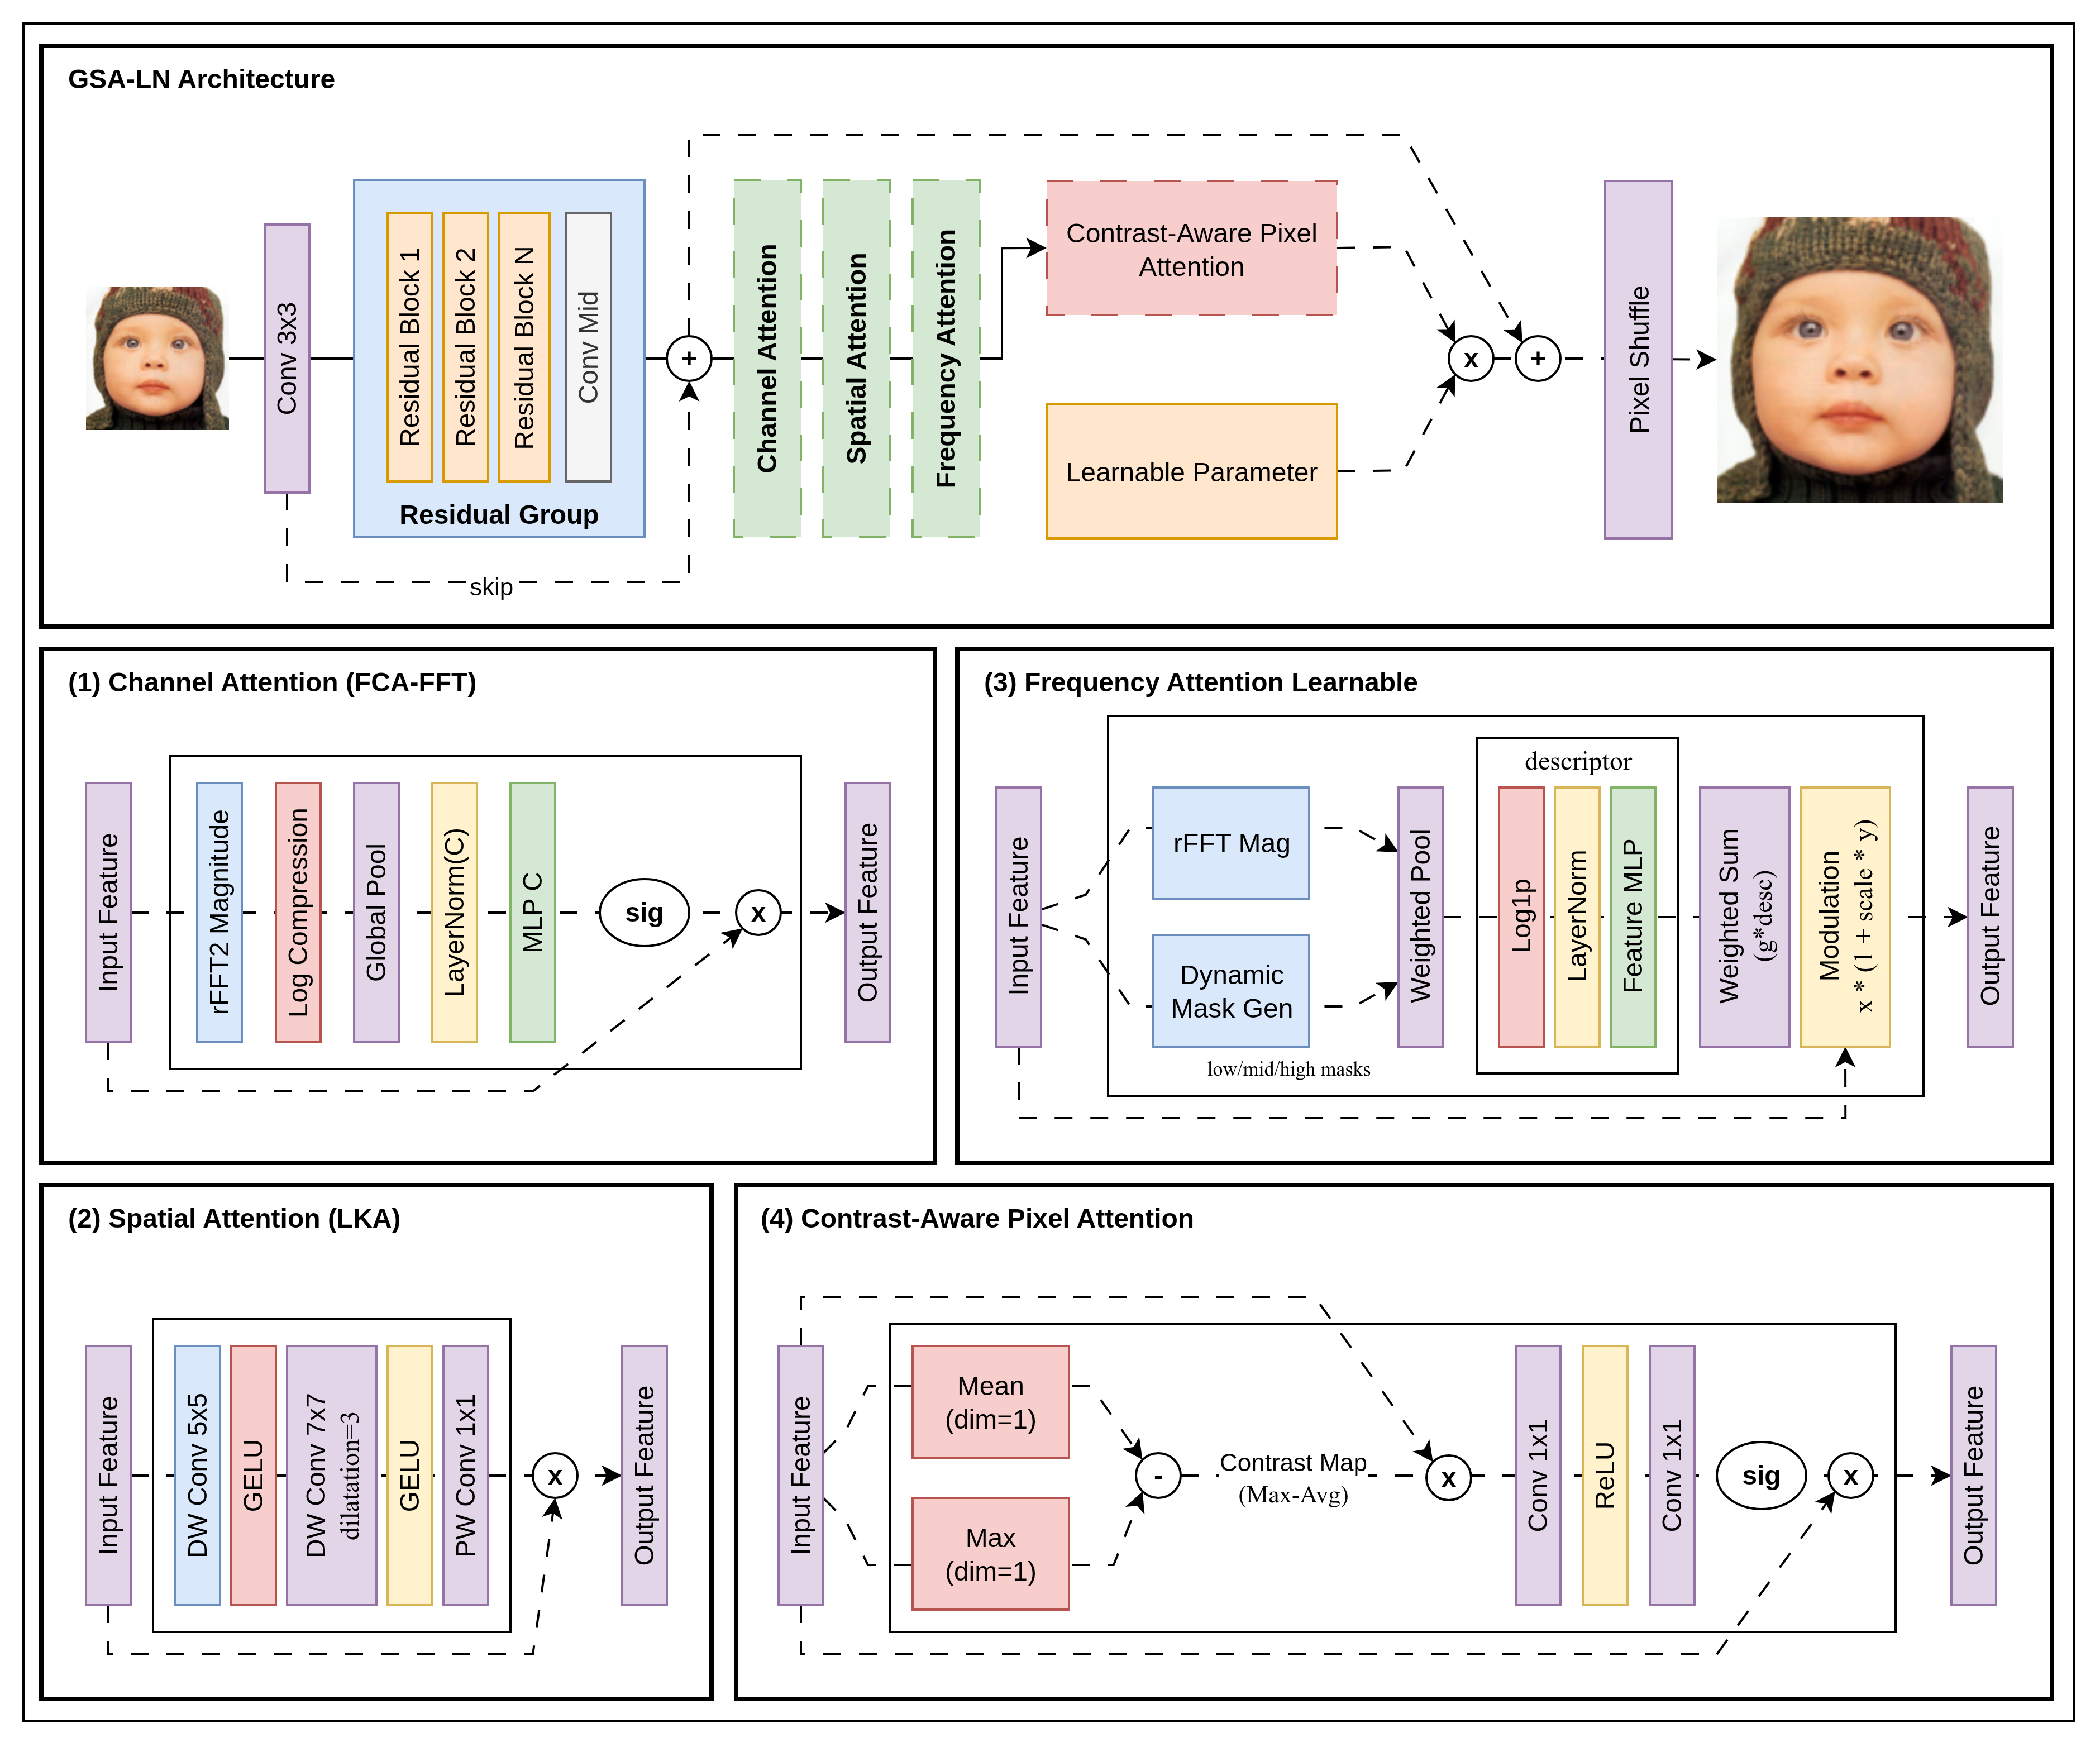
\includegraphics[width=0.95\textwidth]{../../figs/arch.png}
    \caption{Overview of the proposed GSA-LN architecture. The model combines a residual backbone, frequency-aware channel attention, decomposed large-kernel spatial attention, learnable frequency attention, contrast-aware pixel refinement, and PixelShuffle reconstruction.}
    \label{fig:architecture}
\end{figure*}

\subsection{Frequency-Aware Channel Attention}

Given an intermediate feature tensor $F \in \mathbb{R}^{C \times H \times W}$, the model computes a two-dimensional real FFT and extracts the magnitude response:
\begin{equation}
M = |\mathcal{F}(F)|.
\end{equation}
A compact channel descriptor is obtained by log-compression and global averaging over the frequency dimensions:
\begin{equation}
d_c = \frac{1}{HW'} \sum_{u,v} \log(1 + M_{c,u,v}),
\end{equation}
where $W'$ is the reduced width in the real FFT representation. The descriptor is normalized with LayerNorm and passed through a two-layer MLP to obtain channel gates:
\begin{equation}
g = \sigma(W_2 \delta(W_1 LN(d))).
\end{equation}
The gated output is computed as:
\begin{equation}
F_{ca} = F \odot g.
\end{equation}

\subsection{Large Kernel Spatial Attention}

To capture wider spatial dependencies without using expensive deformable or global attention operations, GSA-LN uses decomposed large kernel attention. The module applies a local depth-wise convolution, a dilated depth-wise convolution, and a point-wise convolution:
\begin{equation}
A_s = H_{1 \times 1}(H_{dw,dilated}(H_{dw,local}(F_{ca}))).
\end{equation}
The spatially modulated feature is:
\begin{equation}
F_{sa} = F_{ca} \odot A_s.
\end{equation}
This design enlarges the receptive field while keeping the operation convolutional and parameter efficient.

\subsection{Learnable Frequency Attention}

The learnable frequency attention module computes spectral magnitude statistics from $F_{sa}$ and assigns soft masks to low-, mid-, and high-frequency regions. Coordinates in the frequency plane are encoded using Fourier feature mapping, then combined with a content descriptor obtained from global average pooling. A small MLP predicts frequency-band masks:
\begin{equation}
[B_l, B_m, B_h] = softmax(H_{mask}([\gamma(u,v), c])),
\end{equation}
where $\gamma(u,v)$ denotes the Fourier-encoded frequency coordinate and $c$ denotes the image-level context descriptor. The masked frequency statistics form a three-band descriptor, which is normalized and projected into modulation weights. The final frequency-aware feature is:
\begin{equation}
F_{fa} = F_{sa} \odot (1 + \alpha A_f),
\end{equation}
where $\alpha$ is a learnable scaling parameter and $A_f$ is the predicted frequency response.

\subsection{Contrast-Aware Pixel Refinement and Residual Scaling}

Before reconstruction, the network applies contrast-aware pixel attention to emphasize high-contrast regions that often contain edges and texture details. The contrast cue is computed from channel-wise average and maximum responses:
\begin{equation}
C(F) = max_c(F) - avg_c(F).
\end{equation}
The refined feature is:
\begin{equation}
F_{ref} = F_{fa} \odot H_{capa}(F_{fa} \odot C(F_{fa})).
\end{equation}
Finally, learnable residual scaling fuses the refined attention feature with the backbone feature:
\begin{equation}
F_{out} = F_{backbone} + s \odot F_{ref},
\end{equation}
where $s$ is a learnable channel-wise scaling parameter initialized to 0.1. The final image is reconstructed with PixelShuffle upsampling.

\section{Experimental Setup}

\subsection{Datasets and Training Configuration}

The model is trained on DF2K, which combines DIV2K and Flickr2K image pairs. Bicubic degradation is used to generate LR-HR training pairs for x2, x3, and x4 scales. The training patch sizes are 192, 288, and 384 for x2, x3, and x4 respectively. Random horizontal flipping and rotation are applied as data augmentation.

Training uses the Adam optimizer with an initial learning rate of $2 \times 10^{-4}$, an L1 reconstruction loss, 600,000 total iterations, 5,000 warm-up iterations, and CosineAnnealingRestartLR with three 200,000-iteration periods. Validation is performed on the Y channel with crop borders corresponding to the scale factor.

\subsection{Evaluation Protocol}

The model is evaluated on Set5, Set14, BSD100, Urban100, and Manga109. PSNR is reported on the luminance channel following the common SISR evaluation protocol. SSIM is used during validation and should be reported in the final version of the manuscript for every dataset and scale.

% TODO: Add complete SSIM table for Set5, Set14, BSD100, Urban100, and Manga109 at x2, x3, and x4.
% TODO: Add inference runtime, FLOPs/MACs, and memory usage. These can be measured by inference only; no retraining is required.
% TODO: Add a numerical ablation table from the W&B comparative ablation report. Do not leave the ablation as narrative only.

\section{Results and Discussion}

\subsection{Parameter Efficiency}

Table \ref{tab:params} summarizes the parameter count of GSA-LN across the three scales. The model remains in the 2.6M to 3.1M parameter range, which supports the efficient multi-scale framing of this study.

\twocolumn[
\begin{@twocolumnfalse}
\centering
\refstepcounter{table}
\label{tab:params}
{\footnotesize \textsc{Table \Roman{table}}\\}
{\footnotesize \textsc{Parameter count of GSA-LN across scales.}\par}
\vspace{0.25\baselineskip}
\begin{tabular}{ccc}
\toprule
Model & Scale & Parameters \\
\midrule
GSA-LN & x2 & 2.6M \\
GSA-LN & x3 & 2.8M \\
GSA-LN & x4 & 3.1M \\
\bottomrule
\end{tabular}
\vspace{0.8\baselineskip}

\refstepcounter{table}
\label{tab:psnr}
{\footnotesize \textsc{Table \Roman{table}}\\}
{\footnotesize \textsc{PSNR and parameter comparison on standard bicubic SISR benchmarks. Rows are sorted from the lowest to highest mean PSNR over Set5, Set14, B100, and U100 within each scale. Blue and red values indicate the best and second-best PSNR, respectively. SwinIR-LW denotes the lightweight SwinIR setting. A dash in Params indicates that a reliable parameter count was not identified from the original source.}\par}
\vspace{0.35\baselineskip}
\tiny
\setlength{\tabcolsep}{2.6pt}
\renewcommand{\arraystretch}{0.74}
\begin{tabular*}{\textwidth}{@{\extracolsep{\fill}}lccccccc}
\toprule
Model & Scale & Params & Set5 & Set14 & B100 & U100 & M109 \\
\midrule
VDSR & x2 & 0.666M & 37.53 & 33.03 & 31.90 & 30.76 & - \\
DPN & x2 & - & 37.52 & 33.08 & 31.89 & 30.82 & - \\
A2F-S & x2 & 0.320M & 37.79 & 33.32 & 31.99 & 31.44 & 38.11 \\
HDRN & x2 & - & 37.75 & 33.49 & 32.03 & 31.87 & 38.07 \\
MADNet & x2 & - & 37.94 & 33.46 & 32.10 & 31.74 & - \\
FALSR-A & x2 & 1.021M & 37.82 & 33.55 & 32.12 & 31.93 & - \\
CBPN & x2 & - & 37.90 & 33.60 & 32.17 & 32.14 & - \\
IMDN & x2 & 0.694M & 38.00 & 33.63 & 32.19 & 32.17 & 38.88 \\
RFDN & x2 & 0.534M & 38.05 & 33.68 & 32.16 & 32.12 & 38.88 \\
\textbf{GSA-LN} & \textbf{x2} & \textbf{2.6M} & \ranksecond{38.14} & 33.78 & 32.26 & 32.56 & \ranksecond{39.19} \\
SwinIR-LW & x2 & 0.878M & \ranksecond{38.14} & 33.86 & 32.31 & 32.76 & 39.12 \\
EDSR & x2 & 43M & 38.11 & \ranksecond{33.92} & \ranksecond{32.32} & \ranksecond{32.93} & 39.10 \\
RCAN & x2 & 16M & \rankfirst{38.27} & \rankfirst{34.12} & \rankfirst{32.41} & \rankfirst{33.34} & \rankfirst{39.44} \\
\midrule
VDSR & x3 & 0.666M & 33.66 & 29.77 & 28.82 & 27.14 & - \\
DPN & x3 & - & 33.71 & 29.80 & 28.84 & 27.17 & - \\
A2F-S & x3 & 0.324M & 34.06 & 30.08 & 28.92 & 27.57 & 32.86 \\
HDRN & x3 & - & 34.24 & 30.23 & 28.96 & 27.93 & 33.17 \\
MADNet & x3 & - & 34.26 & 30.29 & 29.04 & 27.91 & - \\
IMDN & x3 & 0.703M & 34.36 & 30.32 & 29.09 & 28.17 & 33.61 \\
RFDN & x3 & 0.541M & 34.41 & 30.34 & 29.09 & 28.21 & 33.67 \\
\textbf{GSA-LN} & \textbf{x3} & \textbf{2.8M} & 34.56 & 30.47 & 29.18 & 28.52 & 34.12 \\
SwinIR-LW & x3 & 0.886M & 34.62 & \ranksecond{30.54} & 29.20 & 28.66 & 33.98 \\
EDSR & x3 & 43M & \ranksecond{34.65} & 30.52 & \ranksecond{29.25} & \ranksecond{28.80} & \ranksecond{34.17} \\
RCAN & x3 & 16M & \rankfirst{34.74} & \rankfirst{30.65} & \rankfirst{29.32} & \rankfirst{29.09} & \rankfirst{34.44} \\
\midrule
VDSR & x4 & 0.666M & 31.35 & 28.01 & 27.29 & 25.18 & - \\
DPN & x4 & - & 31.42 & 28.07 & 27.30 & 25.52 & - \\
A2F-S & x4 & 0.331M & 31.87 & 28.36 & 27.41 & 25.58 & 29.77 \\
MADNet & x4 & - & 32.11 & 28.52 & 27.52 & 25.89 & - \\
IMDN & x4 & 0.715M & 32.21 & 28.58 & 27.56 & 26.04 & 30.45 \\
HDRN & x4 & - & 32.23 & 28.58 & 27.53 & 26.09 & 30.43 \\
RFDN & x4 & 0.550M & 32.24 & 28.61 & 27.57 & 26.11 & 30.58 \\
CBPN & x4 & - & 32.21 & 28.63 & 27.58 & 26.14 & - \\
\textbf{GSA-LN} & \textbf{x4} & \textbf{3.1M} & 32.34 & 28.73 & 27.65 & 26.33 & 30.89 \\
SwinIR-LW & x4 & 0.897M & 32.44 & 28.77 & 27.69 & 26.47 & 30.92 \\
EDSR & x4 & 43M & \ranksecond{32.46} & \ranksecond{28.80} & \ranksecond{27.71} & \ranksecond{26.64} & \ranksecond{31.02} \\
RCAN & x4 & 16M & \rankfirst{32.63} & \rankfirst{28.87} & \rankfirst{27.77} & \rankfirst{26.82} & \rankfirst{31.22} \\
\bottomrule
\end{tabular*}
\vspace{0.8\baselineskip}
\end{@twocolumnfalse}
]

\subsection{Quantitative Comparison}

Table \ref{tab:psnr} reports PSNR values on five standard SISR benchmarks. To keep the comparison more balanced, the table includes early CNN baselines, strong high-capacity CNN/attention models, lightweight CNN models, and a lightweight transformer baseline. The published baseline values are taken from the corresponding SISR papers and their reported bicubic Y-channel evaluations \cite{kim2016vdsr,lim2017edsr,zhang2018rcan,hui2019imdn,liu2020rfdn,liang2021swinir,lan2021madnet,chu2021falsr,zhu2019cbpn,jiang2020hdrn,wang2020a2fs}. The results show that GSA-LN obtains competitive reconstruction quality across scales while maintaining a compact parameter budget. The improvement trend is especially visible on Set5 and Manga109, where high-frequency structures and strong edges benefit from the combination of spectral and spatial attention.

\subsection{Set5 Validation SSIM}

Table \ref{tab:set5_ssim} reports the best Set5 validation PSNR and SSIM values obtained from the training logs. These values are included to summarize structural reconstruction consistency across scale factors. Since the currently available SSIM records are limited to Set5 validation, the multi-dataset comparison in Table \ref{tab:psnr} is kept as PSNR-only.

\begin{table}[H]
\centering
\caption{Best Set5 validation PSNR and SSIM across scales.}
\label{tab:set5_ssim}
\begin{tabular}{ccc}
\toprule
Scale & PSNR & SSIM \\
\midrule
x2 & 38.14 & 0.9609 \\
x3 & 34.56 & 0.9284 \\
x4 & 32.34 & 0.8967 \\
\bottomrule
\end{tabular}
\end{table}

\subsection{Discussion}

The results suggest that GSA-LN is more appropriately described as an efficient and competitive SISR model rather than a universal state-of-the-art method. This distinction is important for a journal submission because transformer-based models and very large restoration networks may obtain stronger absolute performance under different training settings. The contribution of GSA-LN is therefore positioned in the practical middle ground: a compact convolutional model that uses spectral-spatial attention to improve reconstruction quality without a large parameter increase.

The 600,000-iteration training budget is interpreted as experimental context rather than as the main basis for comparison. Published SISR baselines use heterogeneous training protocols, ranging from 9,960 iterations for VDSR to approximately one million updates for EDSR, RCAN, and IMDN \cite{kim2016vdsr,lim2017edsr,zhang2018rcan,hui2019imdn}, so the primary comparison remains focused on reconstruction accuracy and model compactness.

The x2 results show the strongest absolute PSNR values, while x3 and x4 remain consistent despite the increased difficulty of larger upscaling factors. Urban100 and Manga109 are particularly useful for evaluating structured textures and repeated patterns. The improvement on these datasets supports the hypothesis that frequency-aware and large-kernel attention can help recover structural details. However, this claim should be further supported by complete SSIM values, visual comparisons, and ablation data.

\subsection{Short-Run Ablation Study}

Table \ref{tab:ablation} reports a short-run ablation study on Set5 x2 at 30,002 training iterations. The experiment compares selected architectural variants under the same early-training budget. The CAPA variant obtains the highest PSNR and SSIM among the tested variants, improving PSNR by 0.53 dB over the EDSR-style baseline. This result motivated the use of CAPA in the full-iteration GSA-LN configuration. Since the ablation is limited to x2, Set5, and short-run training, it is interpreted as component-level evidence rather than a full convergence comparison.

\begin{table}[H]
\centering
\caption{Short-run ablation on Set5 x2 at 30,002 iterations.}
\label{tab:ablation}
\scriptsize
\setlength{\tabcolsep}{2.8pt}
\begin{tabular}{lrrrr}
\toprule
Variant & Params & $L_1$ loss & PSNR & SSIM \\
\midrule
EDSR baseline & 429,552 & 0.016005 & 35.1594 & 0.9475 \\
HFA+CAPA & 483,424 & 0.015817 & 35.5130 & 0.9472 \\
FourierContentAware & 518,178 & 0.015784 & 35.5949 & 0.9476 \\
Learnable MLP & 434,147 & 0.015796 & 35.6351 & 0.9480 \\
CAPA & 515,379 & \textbf{0.015757} & \textbf{35.6895} & \textbf{0.9483} \\
\bottomrule
\end{tabular}
\end{table}

\section{Limitations}

This study is limited to bicubic SISR degradation and standard benchmark datasets. Therefore, the results should not be interpreted as evidence of robustness under real-world sensor degradation, compression artifacts, or remote sensing conditions. A more complete evaluation should include complete multi-dataset SSIM reporting, runtime analysis, FLOPs/MACs measurement, and full-convergence ablation across more scale factors. These additions can be obtained from inference and controlled component experiments without changing the main training domain.

\section{Conclusion}

This paper reframes GSA-LN as an efficient LayerNorm-gated spectral-spatial attention network for multi-scale SISR. The model combines a batch-normalization-free residual backbone, FFT-based channel descriptors, decomposed large-kernel spatial attention, learnable frequency attention, CAPA, and learnable residual scaling. Experiments on standard bicubic SISR benchmarks show competitive PSNR values across x2, x3, and x4 scales with only 2.6M to 3.1M parameters. The results support the use of spectral-spatial attention for compact SISR models, while the remaining work should focus on complete SSIM reporting, runtime/FLOPs analysis, and rigorous numerical ablation.

\begin{thebibliography}{00}

\bibitem{dong2016srcnn}
C. Dong, C. C. Loy, K. He, and X. Tang, ``Image super-resolution using deep convolutional networks,'' \emph{IEEE Transactions on Pattern Analysis and Machine Intelligence}, vol. 38, no. 2, pp. 295--307, 2016.

\bibitem{kim2016vdsr}
J. Kim, J. K. Lee, and K. M. Lee, ``Accurate image super-resolution using very deep convolutional networks,'' in \emph{Proceedings of the IEEE Conference on Computer Vision and Pattern Recognition}, 2016, pp. 1646--1654.

\bibitem{lim2017edsr}
B. Lim, S. Son, H. Kim, S. Nah, and K. M. Lee, ``Enhanced deep residual networks for single image super-resolution,'' in \emph{Proceedings of the IEEE Conference on Computer Vision and Pattern Recognition Workshops}, 2017, pp. 1132--1140.

\bibitem{zhang2018rcan}
Y. Zhang, K. Li, K. Li, L. Wang, B. Zhong, and Y. Fu, ``Image super-resolution using very deep residual channel attention networks,'' in \emph{Proceedings of the European Conference on Computer Vision}, 2018, pp. 286--301.

\bibitem{liu2020nlsn}
Y. Liu, W. Tang, and Y. Wu, ``NLSN: Non-local sparse network for image restoration,'' in \emph{Proceedings of the IEEE/CVF Conference on Computer Vision and Pattern Recognition}, 2020, pp. 7133--7142.

\bibitem{liang2021swinir}
J. Liang, J. Cao, G. Sun, K. Zhang, L. Van Gool, and R. Timofte, ``SwinIR: Image restoration using Swin Transformer,'' in \emph{Proceedings of the IEEE/CVF International Conference on Computer Vision Workshops}, 2021, pp. 1833--1844.

\bibitem{hui2019imdn}
Z. Hui, X. Gao, Y. Yang, and X. Wang, ``Lightweight image super-resolution with information multi-distillation network,'' in \emph{Proceedings of the ACM International Conference on Multimedia}, 2019, pp. 2024--2032.

\bibitem{liu2020rfdn}
J. Liu, J. Tang, and G. Wu, ``Residual feature distillation network for lightweight image super-resolution,'' arXiv preprint arXiv:2009.11551, 2020.

\bibitem{lan2021madnet}
R. Lan, L. Sun, Z. Liu, H. Lu, C. Pang, and X. Luo, ``MADNet: A fast and lightweight network for single-image super resolution,'' \emph{IEEE Transactions on Cybernetics}, vol. 51, no. 3, pp. 1443--1453, 2021.

\bibitem{chu2021falsr}
X. Chu, B. Zhang, H. Ma, R. Xu, and Q. Li, ``Fast, accurate and lightweight super-resolution with neural architecture search,'' in \emph{Proceedings of the International Conference on Pattern Recognition}, 2021, pp. 9015--9022.

\bibitem{zhu2019cbpn}
F. Zhu and Q. Zhao, ``Efficient single image super-resolution via hybrid residual feature learning with compact back-projection network,'' in \emph{Proceedings of the IEEE International Conference on Computer Vision Workshops}, 2019, pp. 2453--2460.

\bibitem{jiang2020hdrn}
K. Jiang, Z. Wang, P. Yi, and J. Jiang, ``Hierarchical dense recursive network for image super-resolution,'' \emph{Pattern Recognition}, vol. 107, 2020, Art. no. 107475.

\bibitem{wang2020a2fs}
X. Wang, Q. Wang, Y. Zhao, J. Yan, L. Fan, and L. Chen, ``Lightweight single-image super-resolution network with attentive auxiliary feature learning,'' arXiv preprint arXiv:2011.06773, 2020.

\end{thebibliography}

\end{document}
